
% \begin{figure}[!t]
% %\vspace*{-2\baselineskip}
% \centering
% \includegraphics[width=3.1in]{figures/platform/eval_plat.jpg}
% %\vspace*{-1.0\baselineskip}
% \caption{Photograph of the Evaluation Platform used. The arduino microcontroller connected to the sensor collects the data, which is analysed by algorithms running on a Raspberry Pi.}
% %\vspace*{-0.25\baselineskip}
% \label{fig:eval_plat}
% \end{figure}

\section{Evaluation}
\label{sec:evaluation}
The evaluation is intended to answer the following questions -- \ca can we detect failures~\ie separate faulty PIR sensors from working ones? and \cb what can we learn about the failure? In other words, can we perform diagnosis that can aid in replacing or repairing the sensor? We answer these questions in practical deployments, % that are described next. Our evaluation consists of the following stages:
each consisting of the following stages:

% We evaluate the PIR sensor dependability framework by performing binary classification using frequency domain technique.
\ca {\bfseries Stage I: Failure Detection} The goal of this stage is to isolate defective, faulty sensors from functional, working sensors. Note that we do not diagnose the failure in this stage \ie the sensors deemed faulty could be so due to multiple, as yet unknown reasons.\\
\hspace*{2ex}\cb {\bfseries Stage II: Failure Diagnosis} In this stage, we diagnose the failure by mapping it to the taxonomy defined in \S\ref{subsec:taxonomy}. Using the taxonomy as a reference, we seek to conclude whether it is the lens, pyroelectric or electronics subsystem that contains the failure.\\
\hspace*{2ex}\cc {\bfseries Stage III: Fine-Grained Fault Analysis} In this stage, we learn details about the failure as precisely as possible. \Eg if we attribute a fault to be Class III failure, we seek to narrow it down to see if it is due to deposition of dust or paper on the lens.


%We note that this is not possible in all cases.
% There are 4 possible cases:
% \ca Sensor is faulty, and obstacle is absent, \cb Sensor is faulty, and obstacle is present,\cc Sensor is working, and obstacle is absent and \cd Sensor is working, and obstacle is present,\\

% Furthermore we used a train to test ratio of 0.7:1 for assessing the performance of our model.


\subsection{Real-world Deployments}
\label{subsec:deployment}

%\hl{I added this as a new subsection for now. You might want to separate the deployment part from the analysis. First present the deployment, then in the other subsections, present the relevant analysis -- Sibin.}

We performed the following \emph{deployments across multiple scenarios and geographic locations,~\viz}  
\ca in the elevator of a building (\S\ref{subsubsec:elevator}), 
\cb in the lobby of a university building (\S\ref{subsubsec:lobby}), \cc in a Starbucks coffee shop (\S\ref{subsubsec:starbucks}), and \cd in a cafeteria (\S\ref{subsubsec:cafeteria}) (India).
%to analyze the flow of human traffic during lunch hours, \cb , \cc deployment in the lobby (Appendix \S\ref{subsubsec:lobby}) of our building in the US to analyze diurnal occupance and . 
The different deployment scenarios \ca -- \cc are shown in {\bfseries Fig.~\ref{fig:pir_deployment_scenario}}, and aim to capture diverse environmental conditions and challenges (heat, dust, humidity~\etc). 
%We deploy different faulty sensors
%
%~\viz dislodging the lens, covering the lens with tape, deforming the lens, spraying oil on the optical filter, spraying dust on the lens and creating short circuit damage on the electronic board
%
We used 15 sensors in total across all our deployments comprising of 5 working sensors and 2 faulty sensors per class. A combination of these was used in each of our deployments. In each of these deployments, we followed the pre-deployment process, as mentioned in \S\ref{sebsec:pre_deploy}, where different types of faulty sensors were deployed for a week to collect its \aout and \cout. This pre-deployment is a one-time process to calculate different time and frequency domain characteristics capturing the physics of \aout. A subset of these sensors used in the pre-deployment was randomly picked in each of the deployments.
%\sout{We deployed several faulty and working sensors} 
These sensors were deployed (\textbf{Fig.~\ref{fig:pir_sensor_failure_photographs}}) %Specifically, we performed our deployment in 2 geographic locations: \ci Deployed in the cafeteria analyse flow and movement of human traffic during lunch hours, and \cii Deployed in the elevator and lobby of a building in country B to analyze diurnal occupancy. Faults are introduced into the sensor by artificially inducing different faults in different sensors. 
over a duration of 3 months and collected data both during times of low occupancy (weekends, late nights) and high occupancy (weekdays, working hours). Note that no auxiliary private data such as audio or video were captured during these deployments. 

\begin{figure}[t!]
	%\vspace*{-2\baselineskip}
	\centering
	% \includegraphics[width=\linewidth]{figures/platform/deployment-scenarios.png}
	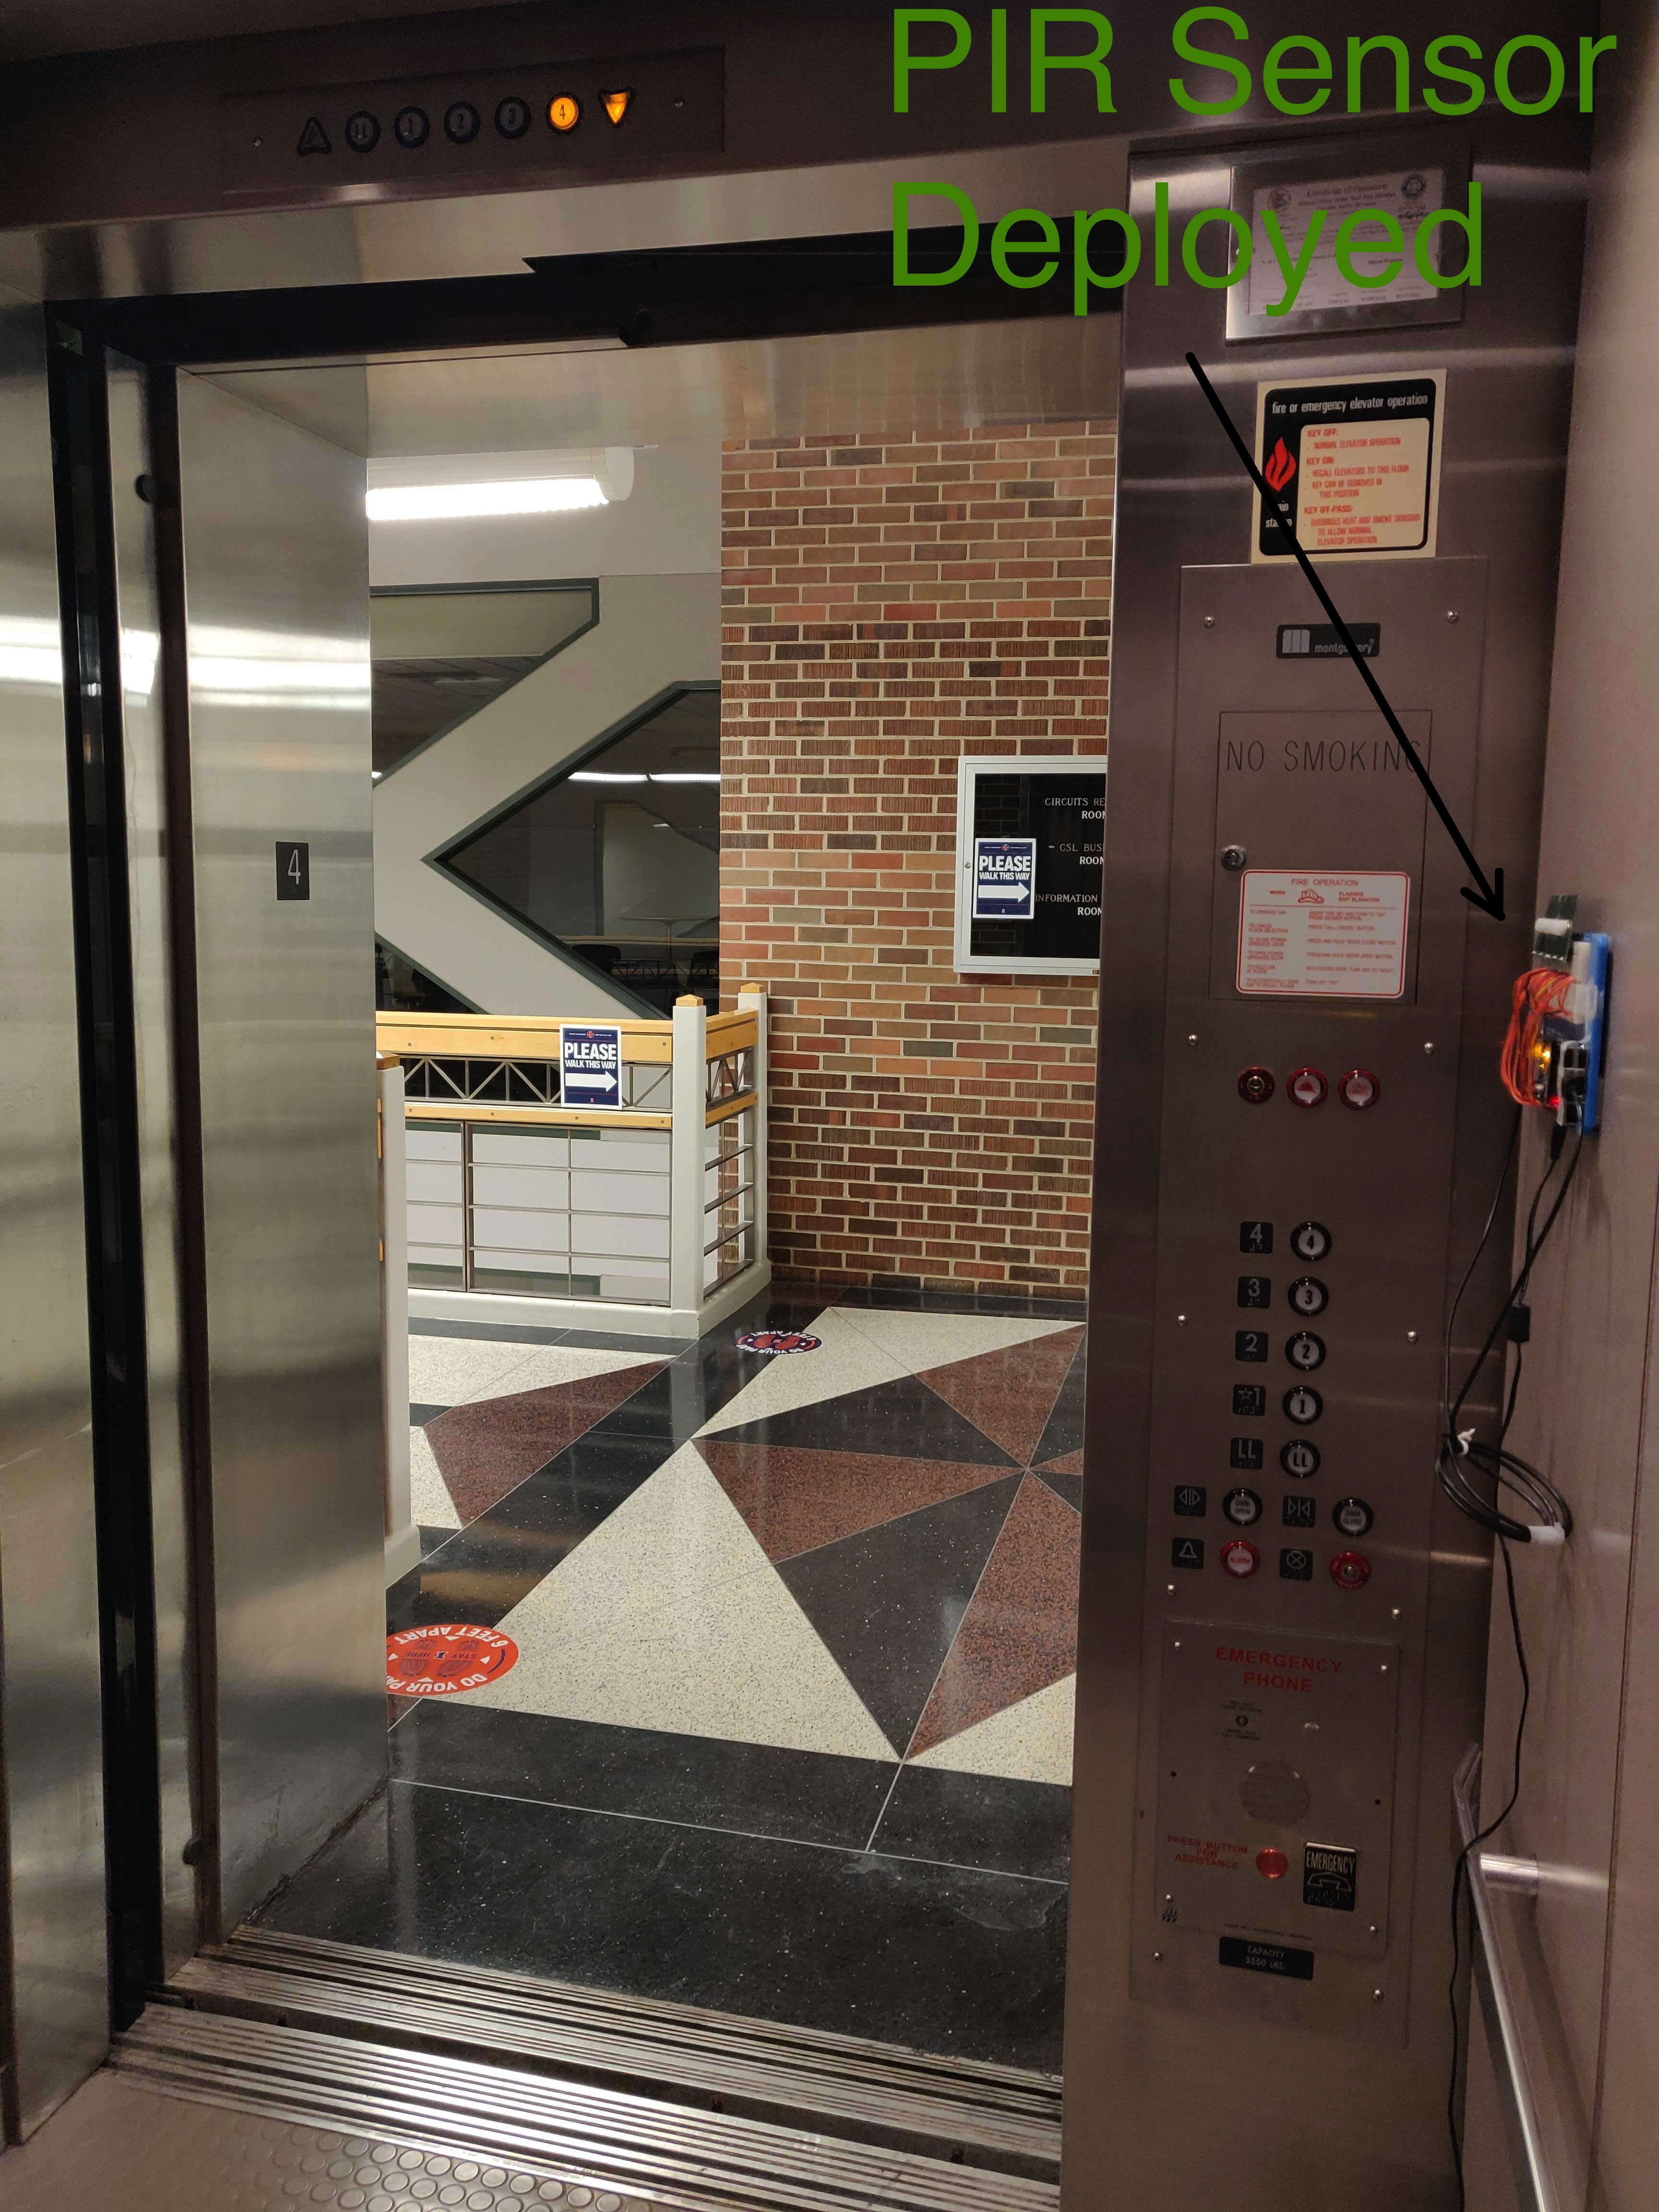
\includegraphics[width=0.3\textwidth, height=1.33in]{figures/deployment/elevator/Elevator-jpg.jpg}
	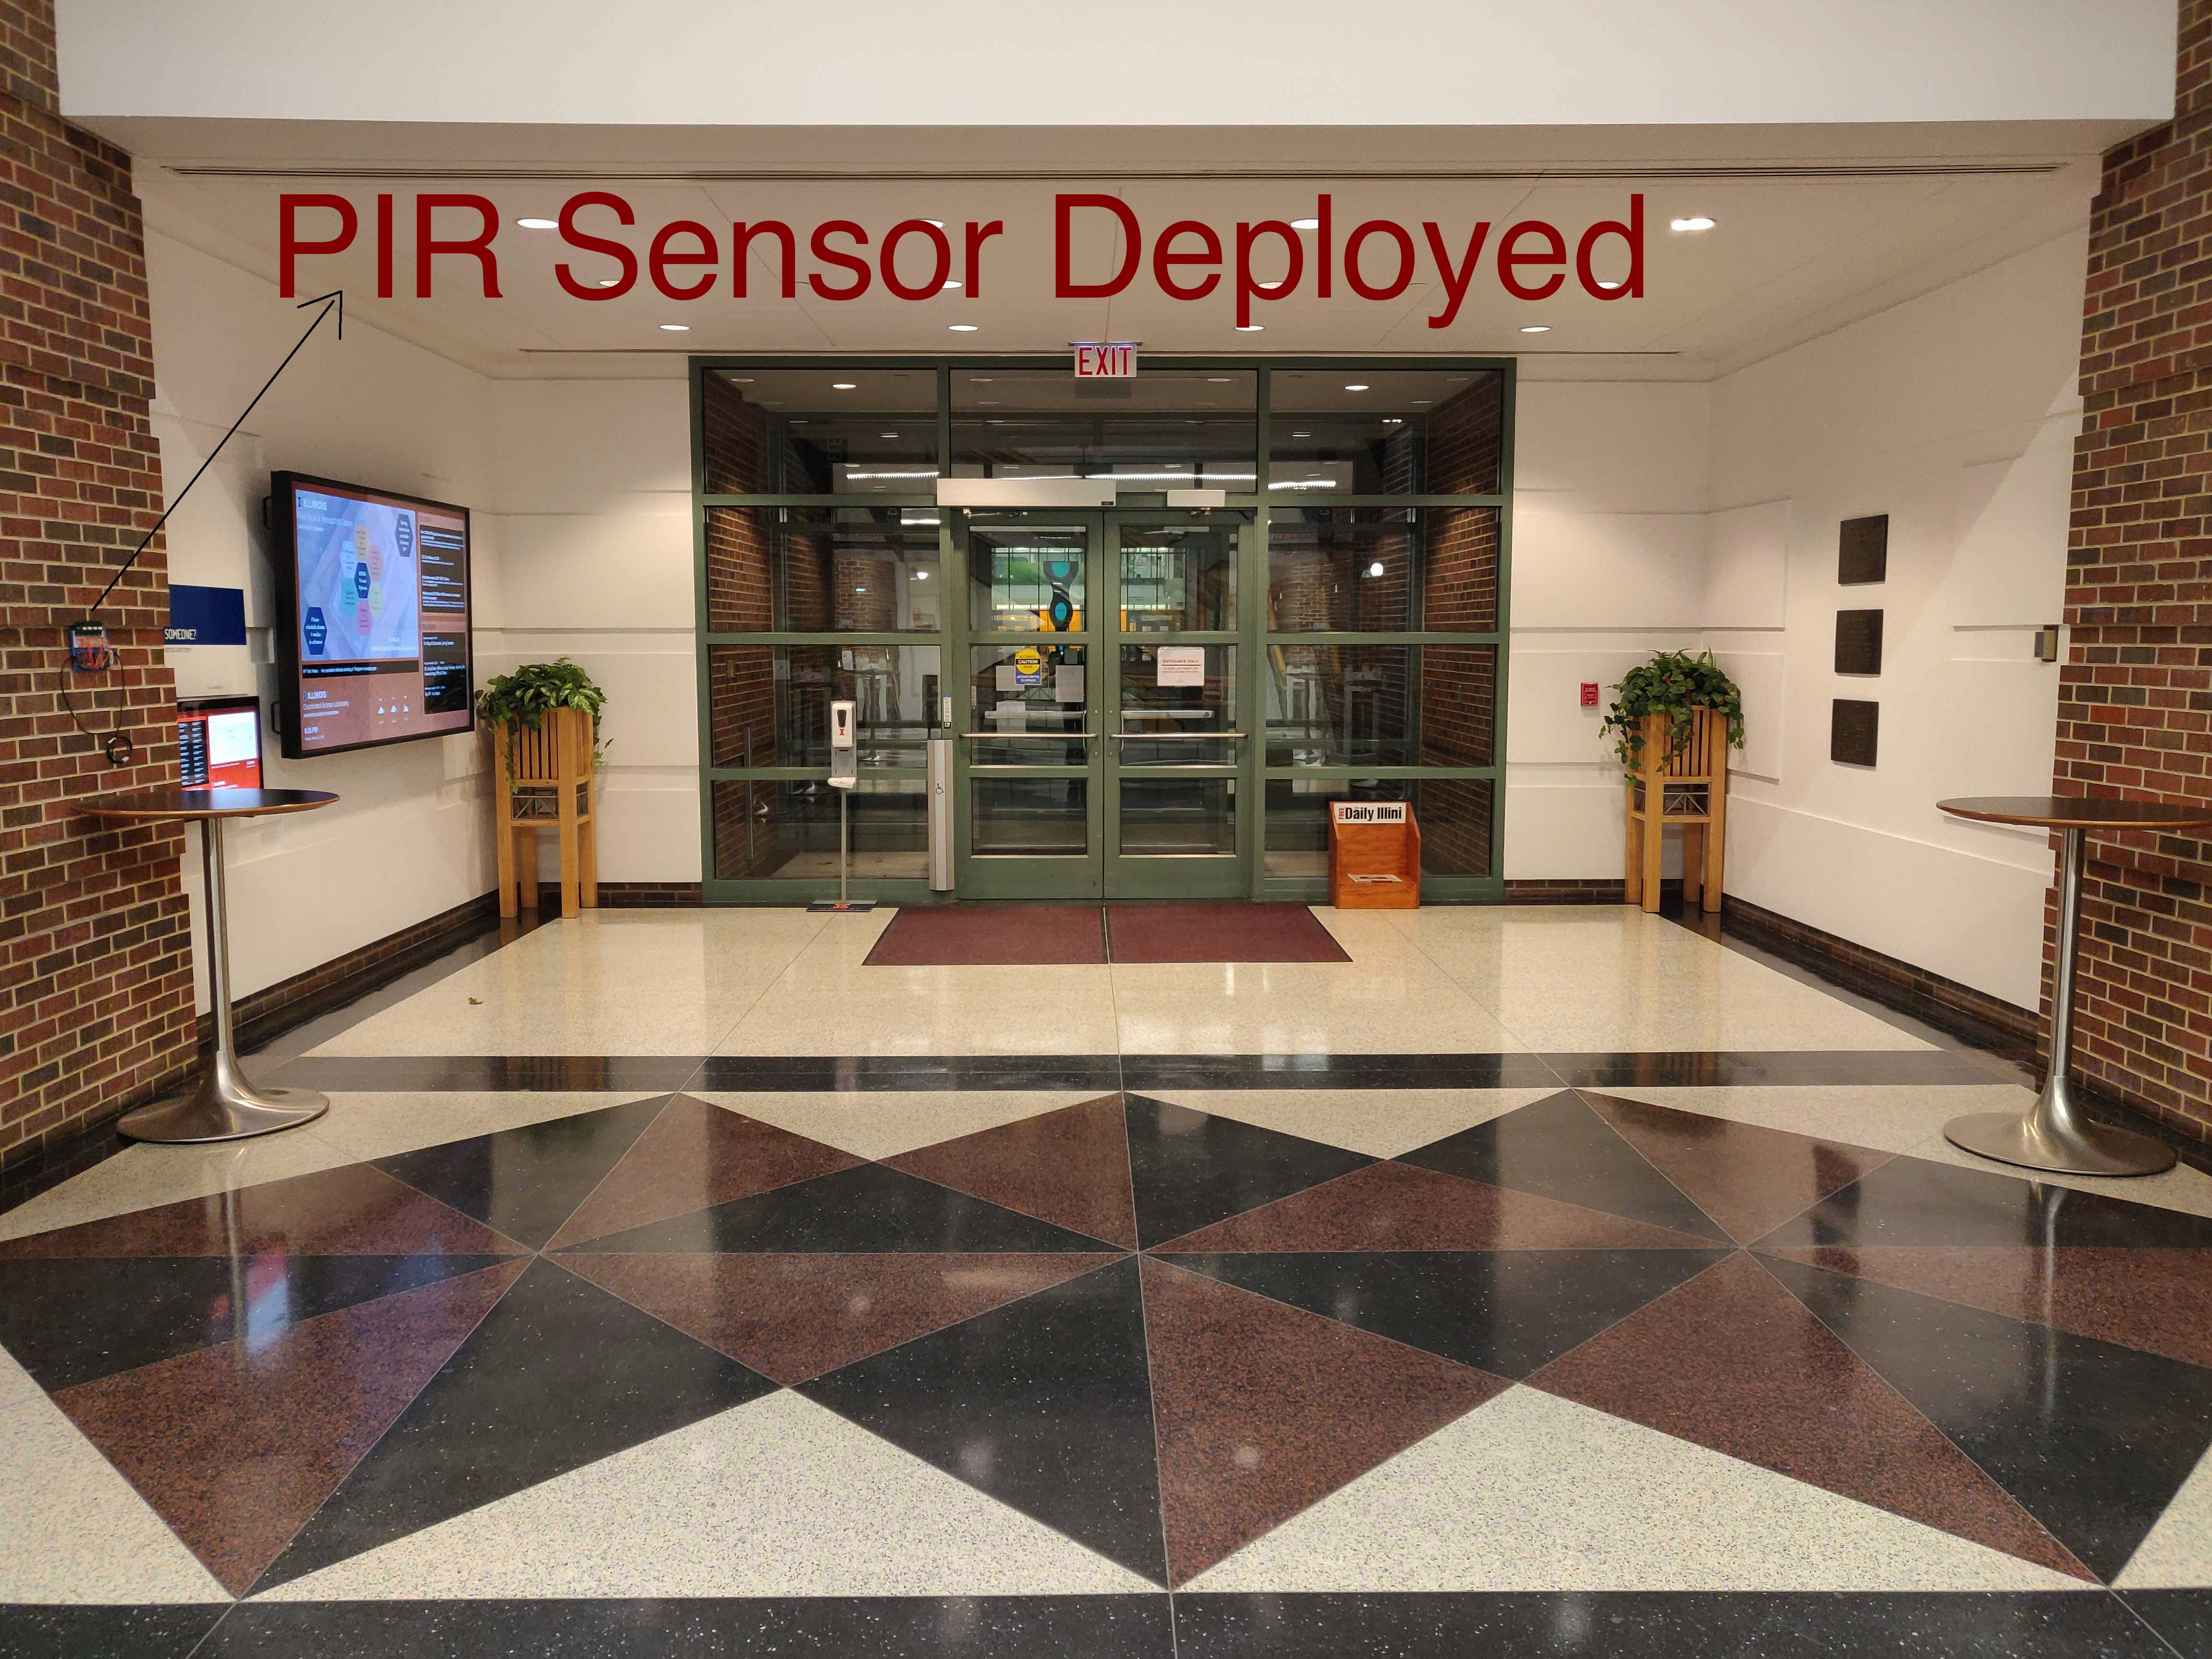
\includegraphics[width=0.3\textwidth]{figures/deployment/lobby/lobby.jpg}
	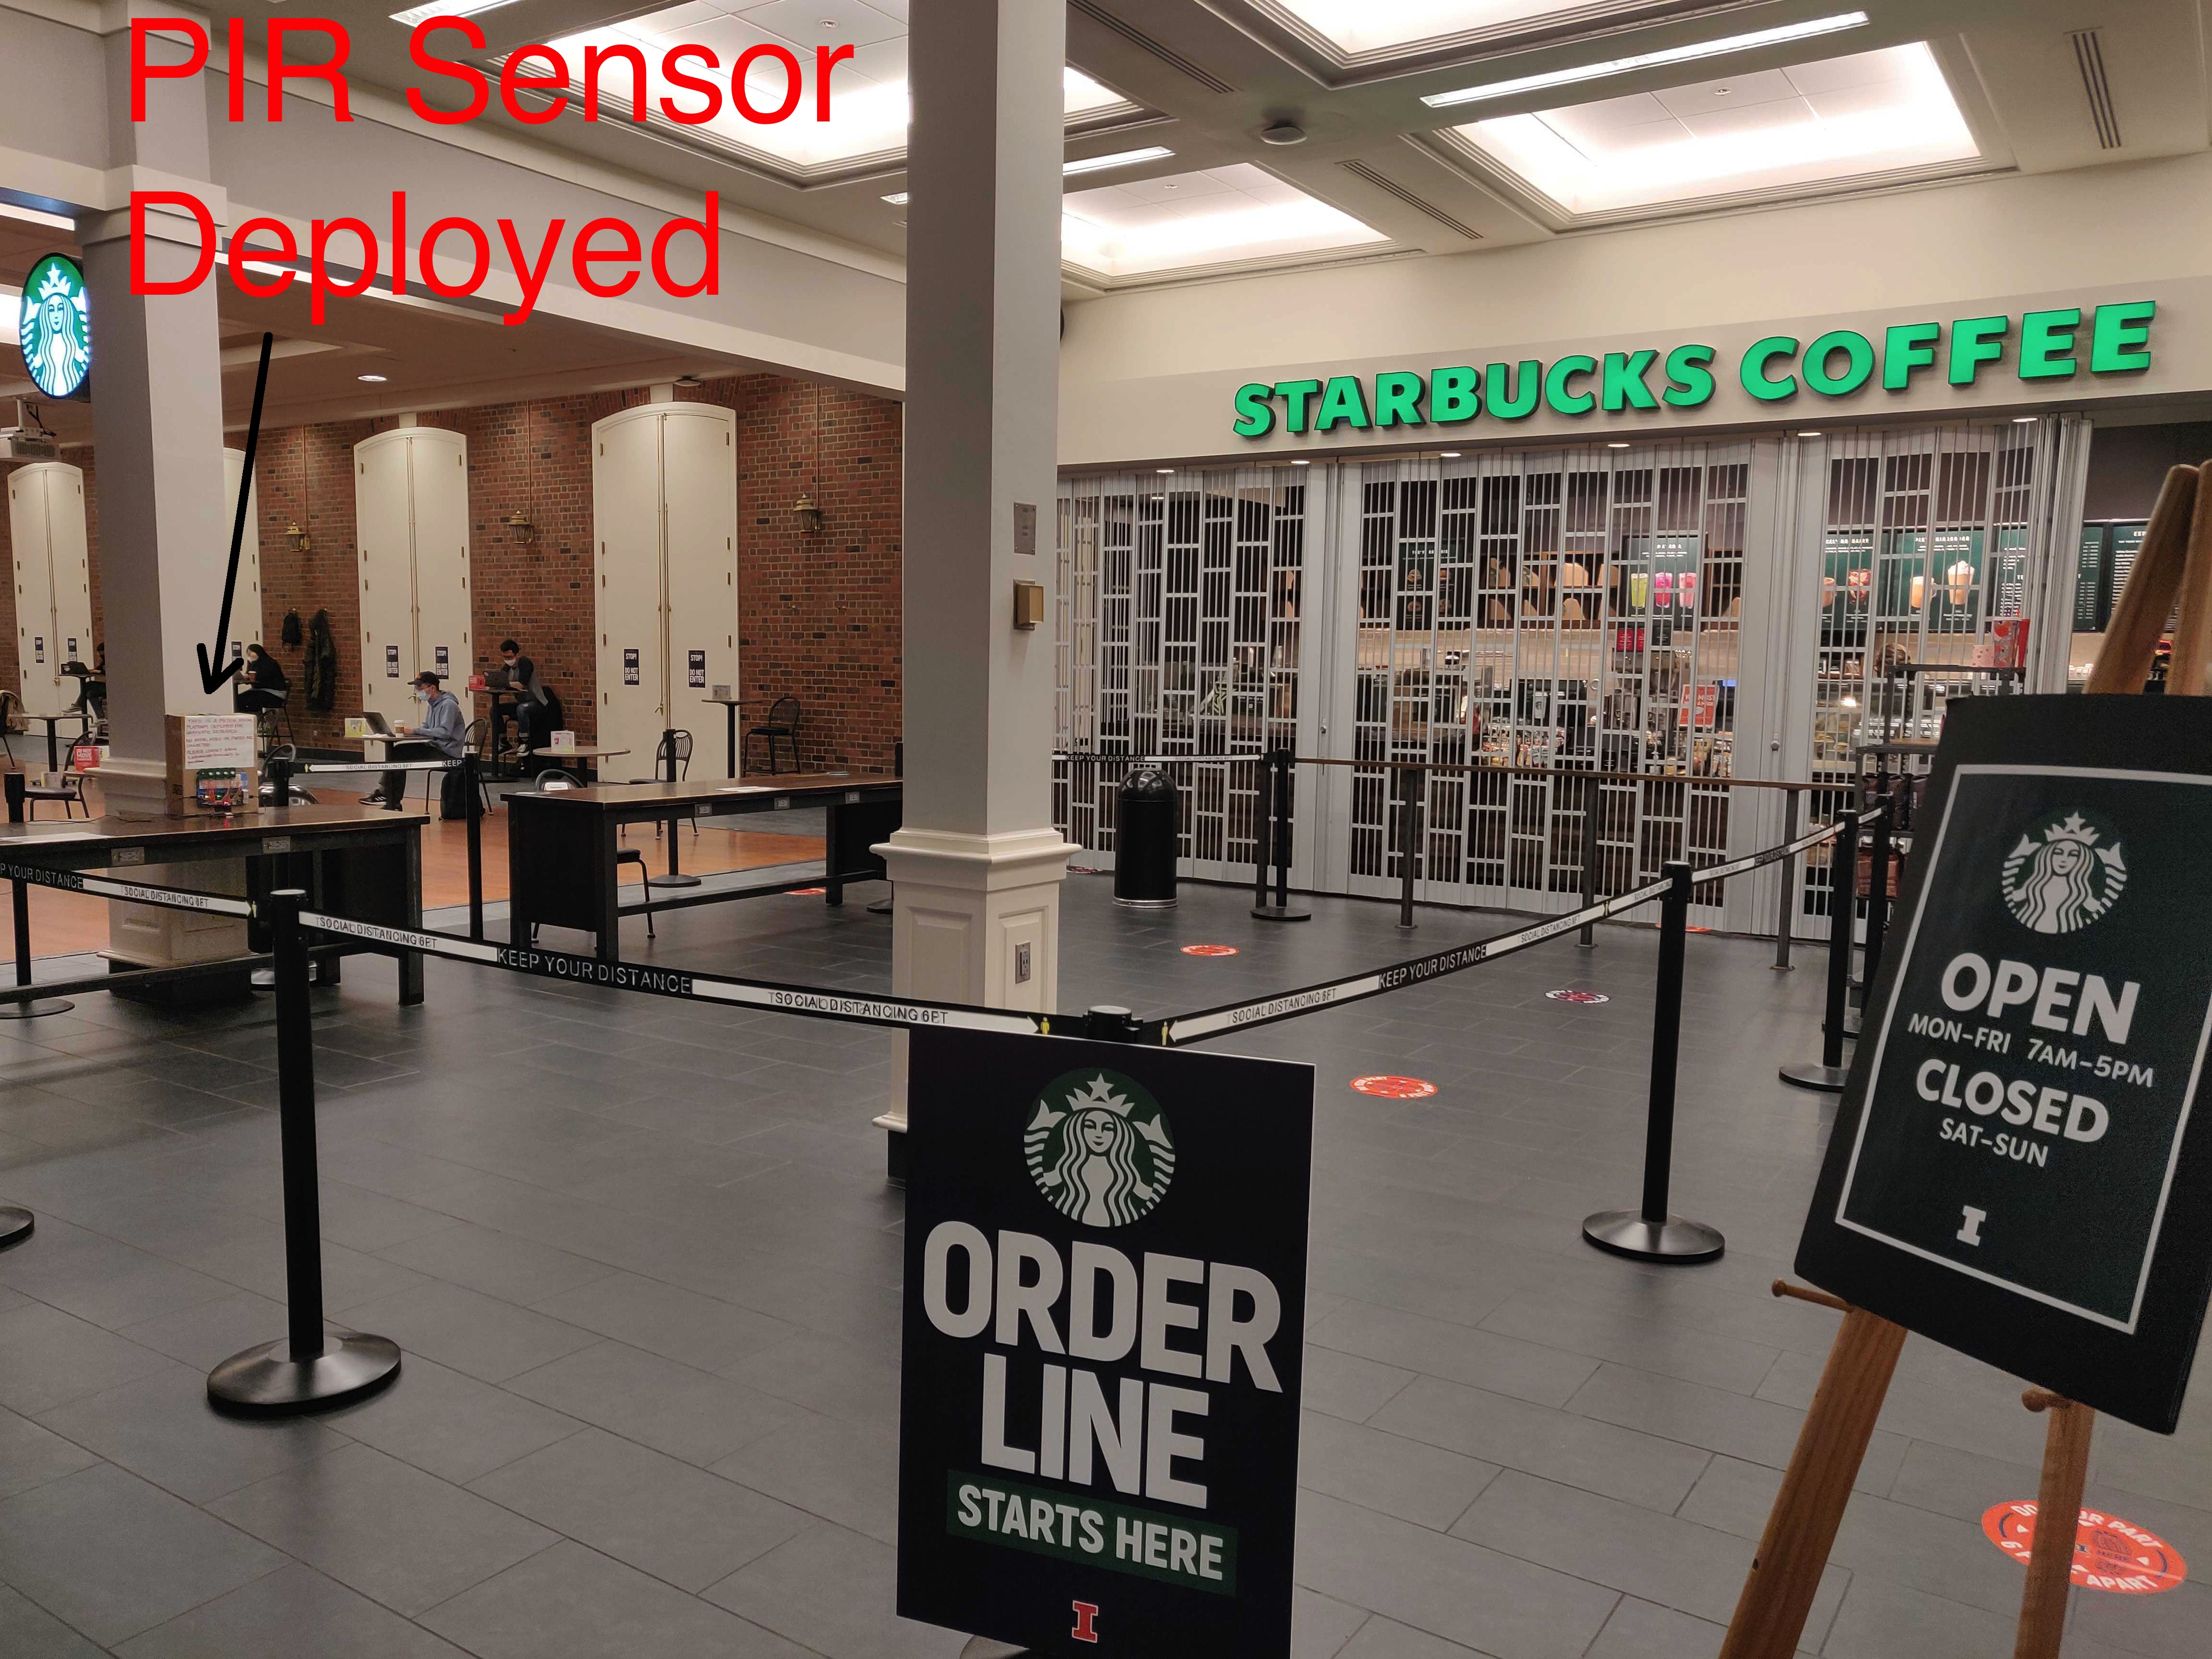
\includegraphics[width=0.3\textwidth]{figures/deployment/coffee_shop/Starbucks-jpg.jpg}
	%\vspace*{-1.0\baselineskip}
		%\vspace{-10pt}
	\caption{\footnotesize{Deployment Scenarios} used for evaluating \sol in PIR sensor failure detection and diagnosis~\viz Elevator, Lobby of a building and Starbucks coffee shop.}
	%\vspace*{-0.25\baselineskip}
	\label{fig:pir_deployment_scenario}
\end{figure}
\begin{figure*}
    \begin{subfigure}[t]{0.4\textwidth}
	%\centering
        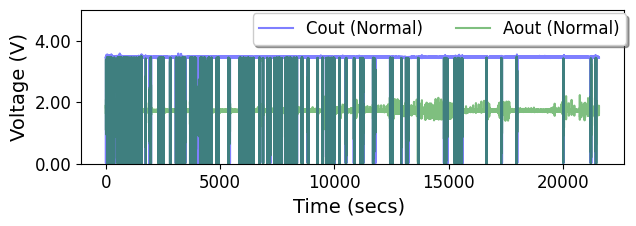
\includegraphics[width=\textwidth]{figures/deployment/elevator/afternoon-6hr.png}
    	%\includegraphics[width=\textwidth]{figures/deployment/elevator/night-8hr.png}%
    	\caption{}
    	\label{fig:deployment_csl_elevator}%
	\end{subfigure}\hfill%
	\begin{subfigure}[b]{0.59\textwidth}
	    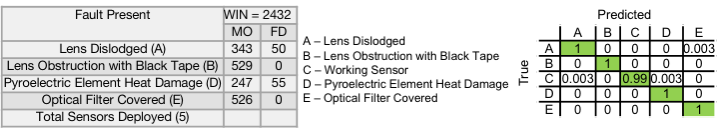
\includegraphics[width=\textwidth, height=0.65in]{figures/deployment/elevator/confusion-matrix-elevator-camera-ready.png}
		\caption{}
		\label{fig:elevator_classification_results}
	\end{subfigure}%
	%\vspace{-15pt}
\caption{\footnotesize Elevator Deployment \ca Occupancy : The graph is a 6 hour deployment during business hours, \cb Deployment Statistics and confusion matrix of the classification model. Column titles: \textbf{WIN}$\rightarrow$Total Number of Windows, \textbf{MO}$\rightarrow$Misses Obstacle, \textbf{FD}$\rightarrow$ False Detection.}
%\vspace{-10pt}
\end{figure*}
\begin{figure*}
	\centering
	\begin{subfigure}[t]{0.4\textwidth}
		\centering
		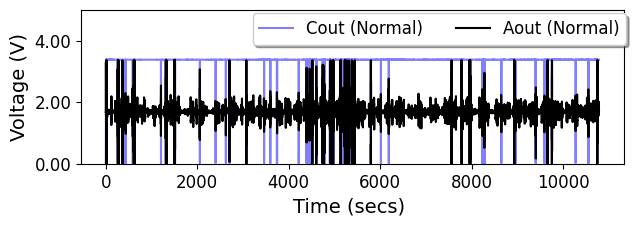
\includegraphics[width=\textwidth]{figures/deployment/lobby/lateafternoon-3hrs.png}
		\caption{}
        \label{fig:deployment_csl_lobby}%
	\end{subfigure}\hfill%
	\begin{subfigure}[b]{0.59\textwidth}
	    \centering
	    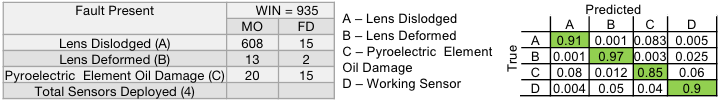
\includegraphics[width=\textwidth]{figures/deployment/lobby/confusion-matrix-lobby-camera-ready.png}
	    %\vspace{-13pt}
	    \caption{}
	    \label{fig:lobby_classification_results}
	\end{subfigure}
	%\vspace{-15pt}
	\caption{\footnotesize Lobby Deployment \ca Occupancy graph during late evening from 6.45 pm to 9.45 pm at the lobby of our university building, \cb Deployment Statistics and confusion matrix of the classification model. Column titles: \textbf{WIN}$\rightarrow$Total Number of Windows, \textbf{MO}$\rightarrow$Misses Obstacle, \textbf{FD}$\rightarrow$ False Detection.} 
	%The confusion matrix on the right shows the predicted label and the true label upon failure analysis.}
	%\vspace{-10pt}
\end{figure*}
\begin{figure*}
	\begin{subfigure}[t]{0.4\textwidth}
		\centering
		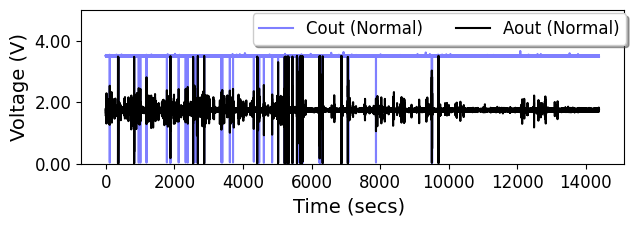
\includegraphics[width=\textwidth]{figures/deployment/coffee_shop/starbucks_4hr_deployment.png}
		%\vspace{-20pt}
		\caption{}
		\label{fig:deployment_starbucks}
	\end{subfigure}\hfill%
	\begin{subfigure}[b]{0.59\textwidth}
	    \centering
	    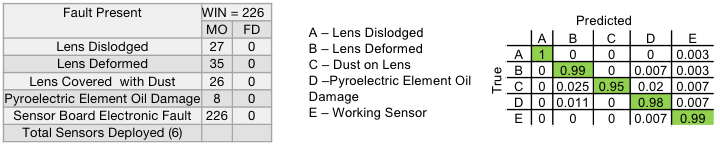
\includegraphics[width=\columnwidth]{figures/deployment/coffee_shop/confusion-matrix-coffeeshop-camera-ready.png}
	    \caption{}
	    \label{fig:coffeeshop_classification_results}
	\end{subfigure}
	%\vspace{-15pt}
	\caption{\footnotesize \textbf{Starbucks Deployment Occupancy}: Evening deployment from 4.45 pm to 8.45 pm. The second half has much lesser little foot traffic. \cb Deployment Statistics and confusion matrix of the classification model. Column titles: \textbf{WIN}$\rightarrow$Total Number of Windows, \textbf{MO}$\rightarrow$Misses Obstacle, \textbf{FD}$\rightarrow$ False Detection. }
	%\vspace{-10pt}
\end{figure*}


%Using the end-to-end characterization described in \S\ref{subsec:high_level_algorithm}, we were able to successfully predict the true labels of the failed sensors. Everytime a failure is detected, we go and manually inspect the sensor to confirm that the sensor is indeed containing a failure. 

%Note that at this stage we did not classify between failed sensors. We obtained the confusion matrix obtained as shown in Table~\ref{tbl:binary_classification_results} using the classifier specification used in deployment is shown in Table~\ref{tbl:binary_classification_classifier_specs}. 

% To verify these results further, we deployed failed sensors, failing it using a mix of different classes of faults and found that we were able to detect failed sensors with an accuracy of 99.85\%.

% We deployed these sensors in the following scenarios -- \ca In an Elevator in a building to detect elevator usage, \cb At a Lobby in a building to capture building occupancy and \cc At Starbucks to capture periods of time with human traffic.

% We studied faults by synthetically creating faulty sensors by injecting the faults into a fraction of sensors and keeping the faulty sensor at certain locations in the building. We observed data from this setup over a period of 2 months, collecting the $A_{out}$ periodically and analysing the Aout for faulty and good sensors.

% When the faults were detected, we went and verified the deployed sensors for the said faults.

% We now look at the specific sensors deployed in each of the scenarios with the goal of identifying the cause of the failure.

%%%%%%%%%%%%%%%%%%%%%%%%%%%%%
% DEPLOYMENT IN ELEVATOR
%%%%%%%%%%%%%%%%%%%%%%%%%%%%%

\subsubsection{Deployment in a University Elevator (US)}\label{subsubsec:elevator} 
%
We deployed working and faulty sensors along the inside wall of an elevator in our university research building (middle {\bfseries Fig.~\ref{fig:pir_deployment_scenario}}). 
%
The data collection captured scenarios of both high and low occupancy during and outside of business hours. % in the building.
%Being pre-pandemic helped us capture scenarios of both high and low occupancy during and outside of business hours in the building.
%
In addition to faulty sensors, we placed a normal, working sensor to keep track of the actual motion in the elevator. 
%
{\bfseries Fig.~\ref{fig:deployment_csl_elevator}} plots \cout and \aout values captured by the working sensor showing the actual traffic in the elevator on one of the days.% when we deployed the sensors. 
%The graph on left is captured during business hours and the graph on right is captured outside business hours. 
Vertical stripes on the graph showing oscillations of \cout (in blue) are points of occupancy \ie denoting a person's entry/exit at the elevator. Likewise, regions of graph with no occupancy is represented by a flat line, hovering around 3.7 V. 

\newcommand{\elevatortable}{% Elevator Deployment Statistics
		\footnotesize
		\centering
		\begin{tabular}{ | l | c | c | }
			\hline
			\multirow{2}{*}{\bfseries \textsc{Fault Present}} & 
			\multicolumn{2}{c|}{\bfseries WIN = 2432} \\
			\cline{2-3}
			& \bfseries MO &  \bfseries FD \\ \hline \hline
			Lens Dislodged &  343 & 50   \\ \hline
			Lens Covered with Black Tape &  529 & 0   \\ \hline
			Pyroelectric Element Heat Damage &  247 &  55 \\ \hline
			Optical Filter Covered & 526 & 0  \\ \hline
			Sensor Board Short & 529 & 0 \\ \hline
		\end{tabular}			
}



% \begin{figure*}
% 	\centering
% 	\begin{minipage}[t]{0.45\textwidth}
% 		\footnotesize
% 		\centering
% 		\begin{tabular}{ | l | c | c | }
% 			\hline
% 			\multirow{2}{*}{\bfseries \textsc{Fault Present}} & 
% 			\multicolumn{2}{c|}{\bfseries WIN = 2432} \\
% 			\cline{2-3}
% 			& \bfseries MO &  \bfseries FD \\ \hline \hline
% 			Lens Dislodged &  343 & 50   \\ \hline
% 			Lens Covered with Black Tape &  529 & 0   \\ \hline
% 			Pyroelectric Element Heat Damage &  247 &  55 \\ \hline
% 			Optical Filter Covered & 526 & 0  \\ \hline
% 			Sensor Board Short & 529 & 0 \\ \hline
% 		\end{tabular}			
% 		\caption{\textbf{Deployment Statistics from Elevator}. Column titles: \textbf{WIN}$\rightarrow$Total Number of Windows, \textbf{MO}$\rightarrow$Misses Obstacle, \textbf{FD}$\rightarrow$ False Detection}
% 		\label{tbl:csl_elevator_deployment}
% 		\hspace{1ex}
% 	\end{minipage}
% 	\begin{minipage}[t]{0.45\textwidth}
% 		\centering
% 		\includegraphics[width=\textwidth]{figures/deployment/elevator/confusion-matrix-elevator.png}
% 		\caption{\textbf{Elevator Deployment} Failure Analysis}
% 		\label{fig:elevator_classification_results}
% 	\end{minipage}
% \end{figure*}

%\textbf{Summary (Figure~\ref{fig:deployment_csl_elevator})} shows a slice of the deployment, where 
%We record the performance of the faulty sensors time windows (of the obstacle) it captured and missed. 
For faulty sensors, we measure the number of time windows where an obstacle was captured or missed. 
%
The performance of faulty sensors relative to a working sensor is tabulated in {\bfseries Fig.~\ref{fig:deployment_csl_elevator}}. 
%The duration of deployment was split into time windows and each window was either classified as '1' (obstacle not present) or '0' (obstacle present) based on the response of the working sensor. We compared each of the faulty sensors with that of the working sensor and calculated \ca False positives ($F_P$) \ie when the working sensor says obstacle not present and the failed sensor says obstacle present and \cb False negative ($F_N$) \ie when the working sensor says obstacle present and the failed sensor says obstacle not present. 
When the lens cap is dislodged, it misses obstacles in 343 time windows whereas the (thermal) breakage of the pyroelectric element results in 247 misses. 
%
Overall, we observe that missed obstacles are more common than false alarms.
%
This ties into common observations in conference rooms operated with PIR sensor-controlled lighting, where lights turn off even with occupants present.


As described in \S\ref{subsec:high_level_algorithm}, \sol collects the \aout signals and uses a machine learning model on their extracted features detect faulty sensors. %FFT coefficients (over a window of 1024 samples). 
%
Using a random forest classifier, we obtain the confusion matrix ({\bfseries Fig.~\ref{fig:elevator_classification_results}}), which shows that predicted label matches the true label for each failure. 
%
We note that -- \ca the working sensor has distinct characteristics compared to the faulty sensors and is isolated correctly, \cb faulty sensors with different failures in lens and pyroelectric subsystem are identified to the failure class correctly as observed by diagonal of the confusion matrix. This implies that the %FFT coefficients 
features of \aout, derived by \sol is able to differentiate between lens being dislodged, lens being covered with tape, oil condensation on the optical filter and heat damage on the pyroelectric element.
%%%%%%%%%%%%%%%%%%%%%%%%%%%%%
% END DEPLOYMENT IN ELEVATOR
%%%%%%%%%%%%%%%%%%%%%%%%%%%%%

%%%%%%%%%%%%%%%%%%%%%%%%%%%%%
% DEPLOYMENT IN LOBBY
%%%%%%%%%%%%%%%%%%%%%%%%%%%%%

% \begin{wrapfigure}{L}{7cm}
% 	\centering
% 	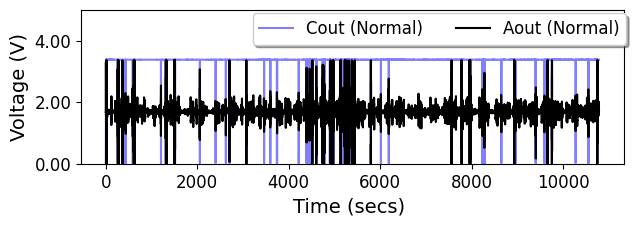
\includegraphics[width=0.49\textwidth]{figures/deployment/lobby/lateafternoon-3hrs.png}
% 	\caption{\textbf{Lobby Deployment Occupancy} : Late evening deployment from 6.45 pm to 9.45 pm at the lobby of a university research building.}
% 	\label{fig:deployment_csl_lobby}
% \end{wrapfigure}

\subsubsection{Deployment in a University Lobby (US)}\label{subsubsec:lobby} We deployed our sensors %The second deployment was 
in the first floor lobby space of our university building. 
%
%Compared to the elevator\footnote{covered in the appendix.} deployment with motion in a restricted direction (entry or exit through same doors), 
The lobby deployment is noisier with fewer constraints on direction of motion, compared to the confined space of an elevator.
% having entry or exit through the same doors. 
%
As in the elevator deployment, we deployed a combination of working and faulty sensors shown in the table in {\bfseries Fig.~\ref{fig:lobby_classification_results}}. 
%The deployment was pre-pandemic, for one week. 



\textbf{Fig.~\ref{fig:deployment_csl_lobby}} shows a 3 hour slice of the deployment. %As explained earlier, 
%
The vertical stripes on \cout correspond to traffic entering/exiting the lobby in the field of view. 
The performance of the sensors deployed, in terms of false detection and missed obstacles, is shown in the table in {\bfseries Fig.~\ref{fig:lobby_classification_results}}. The sensors with lens dislodged missed a large amount of obstacles. This is due to the lack of focus of thermal radiation on the pyroelectric element resulting in dispersion of radiation due to the large lobby area. As a result of this failure, only obstacles that line up in the reduced field of view, are captured. This issue is not present in an elevator due to its confined space.
%
Other faults such as lens deformation and damage due to oil condensation experienced lesser number of misclassifications. 
Upon extracting the features of the \aout signals, and classifying it using the procedure in \S\ref{subsec:high_level_algorithm}, %the same process as described in case of the elevator deployment, 
we observe the confusion matrix as shown in {\bfseries Fig.~\ref{fig:lobby_classification_results}}. The high fraction along the diagonal shows that a majority of sensor failures are classified and identified correctly, as the features are able to bring out differences in the physics of failures.
%Note that compared to the elevator, we observe slightly diminished performance when it comes to fault identification. 
Note that we observe some misclassifications of sensor faults (\eg for C). We argue that this is due to the deployment area of a lobby being open and the limited coverage area of the sensor, both of which can lead to imperfect capture at the periphery. Consequently, for traffic at the edges of field of view, this reduced thermal radiations could lead to some misclassifications. %between a working sensor, a lens deformed/dislodged cases and an oil damage scenario 
% as the sensing process is not activated enough to stress the differences in their physics.

%damage to the pyroelectric element due to humidity is more likely in closed enclosures and the open, well-ventilated conditions of the lobby reduces the condensation due to humidity over time causing to it being misidentified either as working sensor or as a sensor without lens cap for a fraction of the time.

%%%%%%%%%%%%%%%%%%%%%%%%%%%%%
% END DEPLOYMENT IN LOBBY
%%%%%%%%%%%%%%%%%%%%%%%%%%%%%

%%%%%%%%%%%%%%%%%%%%%%%%%%%%%
% DEPLOYMENT IN STARBUCKS QUEUE
%%%%%%%%%%%%%%%%%%%%%%%%%%%%%

\subsubsection{Deployment in a Starbucks (US)}\label{subsubsec:starbucks} 
%
We deployed PIR sensors near the ordering queue of the coffee shop during business hours to capture the typical foot traffic (left {\bfseries Fig.~\ref{fig:pir_deployment_scenario}}). 
%The sensors were placed near the ordering queue. 
%This 
Our deployment %helped us 
captured linear, regularized bidirectional movement (entry followed by exit of the region of interest) ({\bfseries Fig.~\ref{fig:deployment_starbucks}}).
%
Our deployment lasted for a duration of 4 hours on a busy Friday evening. 
%We use a window size of 1024 samples, and look for the number of misclassifications, both false negatives and false positives.  
We observed that out of 226 time windows (each containing 1024 samples), there were missed obstacles across: \ci 27 windows in class I, \cii 35 windows in class II, \ciii 26 windows in class III and no windows in class IV. 
%
The missed obstacles and false detection (none in this case) are summarized in {\bfseries Fig.~\ref{fig:coffeeshop_classification_results}}. 
%
Using \sol, we observe high fractions along the diagonal of the confusion matrix; hence the predicted label of sensor failure matches the true label.
%Note that the oil impurity is not extensive enough to be captured as a fault in the sensor but it still alters the physics of the sensor as described below.

% We collected data from this deployment, extracted features and analyzed using PIRMedic to obtain the confusion matrix as shown in Figure~\ref{fig:coffeeshop_classification_results}. 
Furthermore, despite the oil impurity not being enough cause it to alter performance, we still classify it is a separate class from the physics point of view due to its different behavior of \aout from that of a working sensor.
%is different from that of a working sensor. 
Thus, in line with the previous deployments, we can use the features of \aout to form a signature of the physics. %Additionally, we pick one of the sensors classified as a class I failure, and plot the FFT of its \aout waveform ({\bfseries Fig.~\ref{fig:classI_cross_check}}). We observe that the class I sensor shows similar characteristics to that seen in {\bfseries Fig.~\ref{fig:classI-V_fault_freq}}.


%%%%%%%%%%%%%%%%%%%%%%%%%%%%%
% END DEPLOYMENT IN STARBUCKS QUEUE
%%%%%%%%%%%%%%%%%%%%%%%%%%%%%

%%%%%%%%%%%%%%%%%%%%%%%%%%%%%
% REPLACING TABLE WITH A FIGURE
%%%%%%%%%%%%%%%%%%%%%%%%%%%%%

% \newcommand\items{5}   %Number of classes
% \arrayrulecolor{white} %Table line colors
% \noindent\begin{tabular}{cm{1.65cm}*{\items}{|E}|}
% \multicolumn{1}{c}{} &\multicolumn{1}{c}{} &\multicolumn{\items}{c}{Predicted} \\ \hhline{~*\items{|-}|}
% \multicolumn{1}{c}{} & 
% \multicolumn{1}{c}{} & 
% \multicolumn{1}{c}{\rot{A}} & 
% \multicolumn{1}{c}{\rot{B}} & 
% \multicolumn{1}{c}{\rot{C}} &
% \multicolumn{1}{c}{\rot{D}} &
% \multicolumn{1}{c}{\rot{E}} \\ \hhline{~*\items{|-}|}
% \multirow{\items}{*}{\rotatebox{90}{Actual}} 
% & 
% & 1   & 0  & 0 & 0  & 0  \\ \hhline{~*\items{|-}|}
% & Lens Cap Deformed (B) & 0   & 0.99  & 0 & 0.0073 & 0.0036  \\ \hhline{~*\items{|-}|}
% & Dust on Lens Cap (C) & 0  & 0.025  & 0.95 & 0.018 & 0.0073   \\ \hhline{~*\items{|-}|}
% & Optical filter Oil Impurity (D)  & 0   & 0.011  & 0 & 0.98 & 0.0073   \\ \hhline{~*\items{|-}|}
% & Working Sensor (E) & 0  & 0   & 0 & 0.0073 & 0.99  \\ \hhline{~*\items{|-}|}
% \end{tabular}



\subsubsection{Deployment in a Cafeteria}\label{subsubsec:cafeteria} To evaluate the analysis of \aout during quiet times, we deployed a mix of 3 types of sensors with lens failures -- lens fallen off, lens covered and some working sensors during the lunch hour at a cafeteria in India. The traffic during lunchtime in the cafeteria is as shown in {\bfseries Fig.~\ref{fig:deployment_msr_cafeteria}}. As these were lens-related failures, we looked at the time-domain characterization of \aout during quiet times to understand the status of lens. The time domain representation of \aout, during a period of no occupancy, is as shown in {\bfseries Fig.~\ref{fig:variance_cap_cases}}. The y-axis is plotted in terms of the 10-bit ADC representations of voltage to highlight the differences. For a 10-bit ADC, 1023 units (\ie $2^{10} - 1$) corresponds to a voltage of 5 V. Therefore, a voltage of 1.8 V corresponds to 340 units. 

We note visually that the noise floor at output of the lens subsystem is higher with the lens dislodged ({\bfseries Fig.~\ref{fig:capoff}}) as compared to both a normal sensor ({\bfseries Fig.~\ref{fig:capon}}) and one with lens covered ({\bfseries Fig.~\ref{fig:capcovered}}). Specifically, we observed a variance of 10 $Volt^2$ when lens was covered, 250 $Volt^2$ when lens was in place and working, and 1500 $Volt^2$ when lens had fallen of completely. Consequently, a low threshold ($T_L$) of 100 $Volt^2$ and a high threshold ($T_H$) of 1000 $Volt^2$ was sufficient to separate between the 3 types of sensors. Note that the variance had to be computed during a quiet period of no traffic in this case. %We cover more complex deployments with more classes of sensors next.

%%%%%%%%%%
%%% MSR CAFETERIA
%%%%%%%%%%%%


%	\begin{minipage}{0.49\textwidth}
%		\centering
%		\includegraphics[width=\textwidth]{figures/deployment/coffee_shop/aout-comparison/classI-working.png}
%		\caption{\textbf{\aout comparison} of the Class I diagnosed sensor showing sharper peaks and reduced sensitivity at the periphery.}
%	\end{minipage}%
%	\hfill
\begin{figure*}
	\begin{minipage}[t]{0.48\textwidth}
		%\centering
		%\begin{figure*}%{L}{5cm}
		%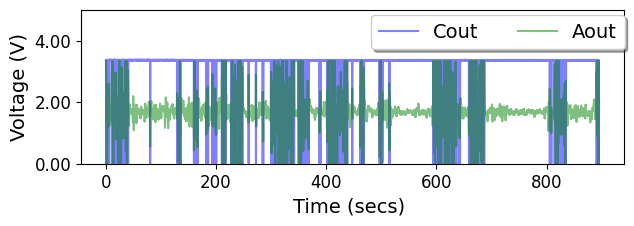
\includegraphics[width=6.75cm]{figures/deployment/bangalore-cafetria/msr-cafeteria-15mins.png}
		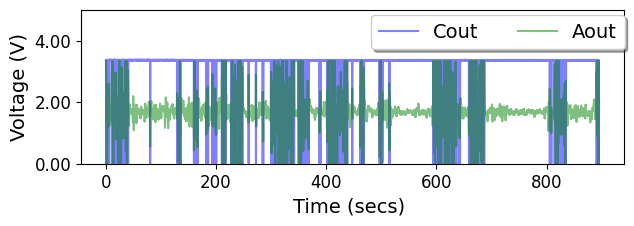
\includegraphics[width=6cm]{figures/deployment/bangalore-cafetria/msr-cafeteria-15mins.png}
		\vspace{-5pt}
		\caption{\textbf{Cafeteria Deployment occupancy} during lunchtime. A 15 min. slice of traffic at the checking counter.}
		\label{fig:deployment_msr_cafeteria}
	\end{minipage}
	\hfill
	\begin{minipage}{0.48\textwidth}
		%\begin{wraptable}{R}{0.6\textwidth}
			\vspace{-\baselineskip}
			%\begin{table}
			%\setlength\tabcolsep{1.45pt}
			%\minipage{0.75\textwidth}
			%\footnotesize
			%\centering
			%\small
			%\hrulefill			
			%\resizebox{\textwidth}{!}{
				%\begin{tabular}{p{2.25cm}p{14.5cm}}
				%\begin{tabular}{p{2cm}p{3.5cm}p{3cm}p{2cm}}
				\begin{tabular}{l c c c c c}
					\hline
					\textbf{Training (MB)} & \textbf{32} & \textbf{64} & \textbf{96} & \textbf{112} & \textbf{128} \\
					\hline \hline
					Accuracy (\%) & 92.4 & 95.8 & 98.6 & 99.1 & 99.4 \\
					\hline
				\end{tabular}
				%}
			\vspace{\baselineskip}
			\caption{\textbf{Failure detection accuracy} as a function of the size of training dataset}
			\label{fig:dataset_size}
			%\vspace*{-1.5\baselineskip}
			%\end{table}
		%\end{wraptable}
	\end{minipage}
\end{figure*}%
%%%%%%%%%%
%%% END MSR CAFETERIA
%%%%%%%%%%%%


%%%%%%%%%%
%%% LENS CAP VARIANCE 
%%%%%%%%%%%%
% ashish
\begin{figure}%[t]
	\centering
	\begin{subfigure}[t]{0.33\linewidth}
		\centering
		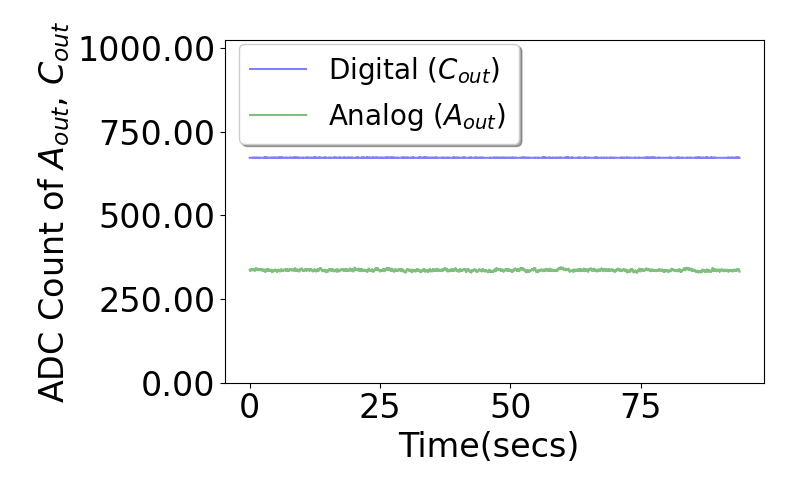
\includegraphics[width=\textwidth]{figures/pir/lens_fault/BuildSys_Graphs/CapCovered_NoObstacle.png}
		\caption{Lens Covered Completely}
		\label{fig:capcovered}
	\end{subfigure}
	\begin{subfigure}[t]{0.33\linewidth}
		\centering
		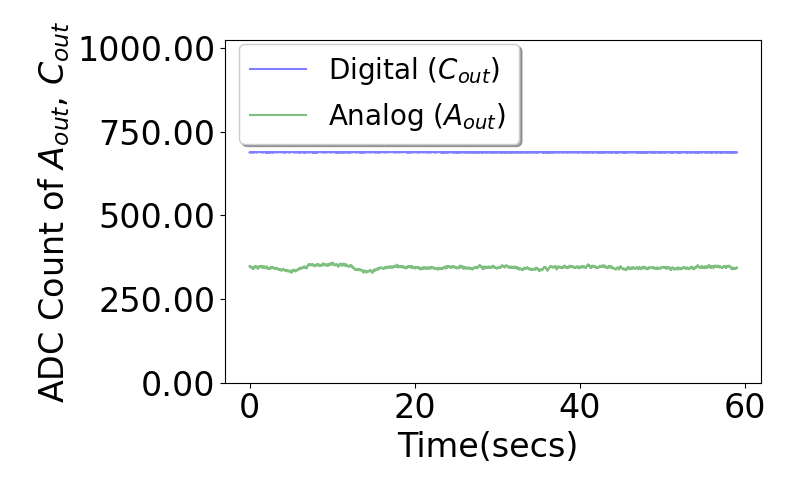
\includegraphics[width=\textwidth]{figures/pir/lens_fault/BuildSys_Graphs/CapON_NoObstacle.png}
		\caption{Lens in Place (Working)}
		\label{fig:capon}
	\end{subfigure}
	\begin{subfigure}[t]{0.33\linewidth}
		\centering
		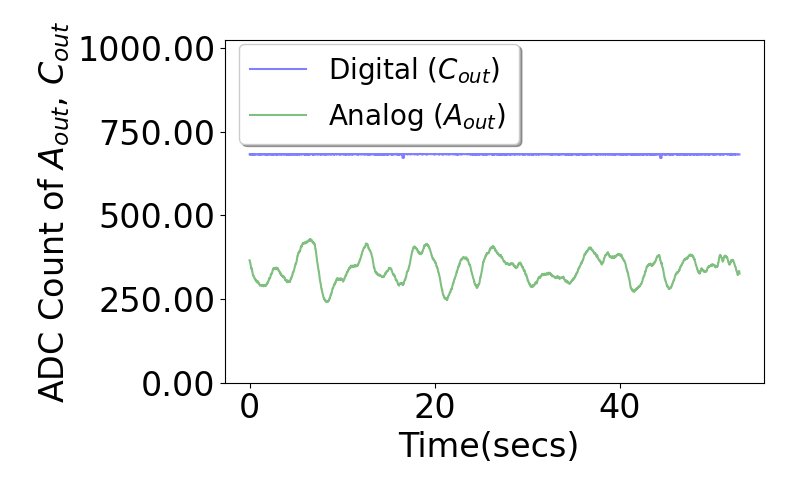
\includegraphics[width=\linewidth]{figures/pir/lens_fault/BuildSys_Graphs/CapOff_NoObstacle.png}
		\caption{Lens Dislodged}
		\label{fig:capoff}
	\end{subfigure}
	\caption{The variance in \aout during known quiet times contains hints about lens failures in the PIR sensor.}
	\label{fig:variance_cap_cases}
\end{figure}

%%%%%%%%%%
%%% END LENS CAP VARIANCE 
%%%%%%%%%%%%


% \subsubsection{Deployment in a cafeteria during Lunch hours} We also deployed the sensor array in a cafeteria setting during lunch hours to capture traffic that is haphazard, disorganized and offering bulk movement. This deployment was done at the cafeteria of a building in Bangalore.
%\vspace{-10pt}

We now discuss the different stages of \sol, as enumerated in the beginning of this section. 

\subsection{Stage I -- Failure Detection}
\label{subsec:fail_detection}

%\hl{note: this section is more about deployment and not about failure detection, yet so moved it here -- Sibin.}

We aggregated all the sensors (both working and faulty) to \textit{separate faulty sensors (without specifying which class) from working sensors}. 
%
We collected FFT coefficients of \aout on a pre-deployment lasting 1 week and performed daily collection of \aout signals from all the deployed sensors. 
%
% Our target is to predict the sensor to be working or faulty, from newly collected FFT features using the PIRMedic algorithm (\S\ref{subsec:high_level_algorithm}). %--\S\ref{subsec:prac}.
%
We used a Random Forest classifier with specifications shown in {\bfseries Fig~\ref{fault_detection_results}}. 
%
%\begin{wraptable}{R}{0.6\textwidth}
%	%\vspace{-\baselineskip}
%	%\begin{table}5
%	%\setlength\tabcolsep{1.45pt}
%	%\minipage{0.75\textwidth}
%	%\footnotesize
%	\centering
%	%\small
%	%\hrulefill
%	\caption{\textbf{Failure detection accuracy vs. the size of training dataset}}
%	%\resizebox{\textwidth}{!}{
%		%\begin{tabular}{p{2.25cm}p{14.5cm}}
%		%\begin{tabular}{p{2cm}p{3.5cm}p{3cm}p{2cm}}
%		\begin{tabular}{l c c c c c}
%			\hline
%			\textbf{Training (MB)} & \textbf{32} & \textbf{64} & \textbf{96} & \textbf{112} & \textbf{128} \\
%			\hline \hline
%			Accuracy (\%) & 92.4 & 95.8 & 98.6 & 99.1 & 99.4 \\
%			\hline 
%		\end{tabular}
%		%}
%	\label{tbl:dataset_size}
%	%\vspace*{-1.5\baselineskip}
%	%\end{table}
%\end{wraptable}
Once predicted, we manually verified the true status of the sensor and observed an accuracy of over 99\% in predicting if the sensor is working or faulty. 
%
Thus, FFT-based features of \aout were able to capture the physics, and hence separate faulty sensor physics from working sensor physics.
%
We also varied the \textit{size of training dataset} (128 MB corresponds to 1 week pre-deployment) to show the robustness of failure detection in {\bfseries Fig.~\ref{fig:dataset_size}}.


\begin{comment}
	\begin{tcolorbox}[left=1pt,right=1pt,top=1ex,bottom=1pt,boxsep=0pt,
		toptitle=0.5ex,bottomtitle=0.5ex]
	{\bfseries Summary:} \ins{The FFT representation of \aout is used to perform binary classification between working and faulty sensors.}
	\end{tcolorbox}
\end{comment} 

%%%%%%%%%%%%%%%%%%%%%%%%%%%%%
% FAILURE DETECTION RESULTS
%%%%%%%%%%%%%%%%%%%%%%%%%%%%%
%\vspace{-10pt}
\begin{wrapfigure}{R}{0.5\textwidth}
	\centering
	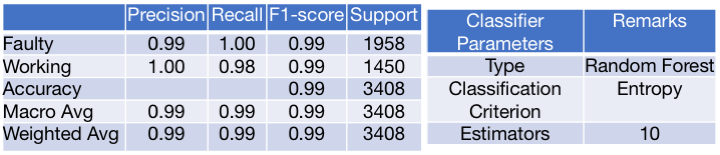
\includegraphics[width=0.5\textwidth]{figures/classification/FaultDetectionResults.png}
	\caption{\footnotesize Fault Detection showing that faulty sensors isolated from working sensors by extracting FFT of \aout and using a Random Forest Classifier.}
	\label{fault_detection_results}
\end{wrapfigure}

%\begin{table}
%	\small
%	\parbox{.45\columnwidth}{
%		\centering
%		\begin{tabular}{l l l}
%			\hline
%			& \bfseries Faulty & \bfseries Working\\ \hline \hline
%			\bfseries Faulty & 99.80 & 0.20 \\
%			\bfseries Working & 1.72 & 98.28  \\ \hline 
%			\rowcolor{gray!20} Overall & 99.15 & \\
%			\hline
%		\end{tabular}
%		\caption{Failure Detection}
%		\label{tbl:binary_classification_results}
%	}
%	%\hfill
%	\hspace{4ex}
%	\parbox{.45\columnwidth}{
%		%\centering
%		\begin{tabular}{l m{1.89cm}}
%			\hline
%			\bfseries Details & \bfseries Remarks\\ \hline \hline
%			Type & Random Forest \\
%			Estimators & 10 \\
%			Criterion & Entropy \\ \hline
%		\end{tabular}
%		\caption{Classifier Details}
%		\label{tbl:binary_classification_classifier_specs}
%	}
%\end{table}

%%%%%%%%%%%%%%%%%%%%%%%%%%%%%
% END FAILURE DETECTION RESULTS
%%%%%%%%%%%%%%%%%%%%%%%%%%%%%